El desarrollo experimental se organizó en cuatro etapas: diagnóstico de la plataforma disponible, diseño y fabricación de las modificaciones, integración del sistema y configuración y calibración de los subsistemas. El procedimiento se planteó de forma iterativa, de manera que cada modificación pudiera verificarse antes de incorporarse a la configuración final.

Como etapa preliminar se rehabilitó una impresora 3D de arquitectura cartesiana perteneciente a la institución, que se encontraba fuera de servicio. Una vez operativa, se utilizó como plataforma de referencia para identificar limitaciones del sistema original y como equipo de apoyo para fabricar los prototipos y componentes poliméricos desarrollados durante el proyecto. La evaluación experimental del sistema final se presenta en el capítulo siguiente


\section{Descripción y diagnóstico de la impresora inicial}
La impresora utilizada como punto de partida corresponde a un sistema de fabricación aditiva por extrusión de material construido sobre perfiles de aluminio. El movimiento de los ejes X y Y se realiza mediante correas dentadas, mientras que el eje Z utiliza dos husillos. Los tres mecanismos son accionados mediante motores paso a paso NEMA 17. La configuración es cartesiana: la cama se desplaza sobre el eje Y y el conjunto de extrusión se posiciona sobre los ejes X y Z.

En su estado original, el equipo utilizaba filamento de diámetro nominal de 3 mm y una boquilla de 0.4 mm. Los componentes del módulo de extrusión estaban sujetos mediante piezas poliméricas y el control se realizaba con una tarjeta RAMPS 1.4. Las dimensiones nominales previstas para el volumen de impresión eran 200 mm en X, 200 mm en Y y 200 mm en Z.

\subsection{Rehabilitación de la impresora}
Debido a que el equipo se encontraba fuera de servicio, se realizó una inspección mecánica, eléctrica y térmica antes de utilizarlo. Los perfiles estructurales, motores, correas y husillos se encontraron en condiciones de operación y se conservaron. En cambio, los controladores de motor no funcionaban y uno de los termistores estaba dañado, por lo que estos componentes fueron sustituidos.

También se identificaron piezas poliméricas deterioradas por envejecimiento. El tensor de la correa del eje Y se fracturó durante la manipulación y fue reemplazado junto con su rodamiento. En el sistema de extrusión se sustituyeron el hotend y la boquilla para utilizar filamento de 1.75 mm. El mecanismo de alimentación original se conservó inicialmente con el propósito de poner en operación el equipo y evaluar su comportamiento.

La versión y configuración del firmware instalado originalmente no pudieron identificarse. Por ello se instaló Marlin 2.1.2.1 y se configuraron nuevamente los parámetros básicos de movimiento, temperatura, extrusión y referencia de los ejes. Después de estas intervenciones, la impresora quedó operativa y pudo utilizarse para el diagnóstico y la fabricación de prototipos.

\subsection{Limitaciones funcionales observadas}

Una vez rehabilitado el equipo se evaluaron las condiciones que podían limitar su ajuste, funcionamiento y posterior utilización como plataforma experimental. La Tabla~\ref{tab:diagnostico_inicial} resume los problemas identificados y el requisito de diseño derivado de cada uno.

\begin{table*}[htbp]
    \centering
    \small
    \caption{Problemas identificados en la configuración inicial.}
    \label{tab:diagnostico_inicial}

    \begin{tabularx}{\textwidth}{
        >{\raggedright\arraybackslash}p{0.16\textwidth}
        Y
        Y
        Y
    }
        \toprule
        \textbf{Subsistema} &
        \textbf{Problema identificado} &
        \textbf{Consecuencia observada o probable} &
        \textbf{Necesidad de diseño} \\
        \midrule

        Módulo de extrusión &
        Deformación del soporte próximo al hotend &
        Pérdida de posición o alineación de los componentes &
        Separar térmicamente el hotend de las piezas poliméricas \\

        \addlinespace

        Enfriamiento &
        Enfriamiento insuficiente o sin conducción dirigida &
        Posible calentamiento de la zona fría del hotend &
        Incorporar ventilación dirigida al disipador \\

        \addlinespace

        Enfriamiento de capa &
        Ausencia de ventilación dirigida hacia la pieza &
        Limitación para controlar el enfriamiento del material depositado &
        Integrar un sistema independiente de enfriamiento de capa \\

        \addlinespace

        Geometría &
        Interferencia del módulo con la estructura &
        Reducción del recorrido y del volumen útil &
        Disminuir las dimensiones exteriores del módulo \\

        \addlinespace

        Estructura &
        Juego mecánico en determinadas uniones &
        Variación en la posición relativa de los componentes &
        Incorporar refuerzos en puntos críticos \\

        \addlinespace

        Transmisión &
        Ausencia de un mecanismo accesible para tensar la correa &
        Dificultad para realizar y reproducir el ajuste &
        Desarrollar un mecanismo de tensión ajustable \\

        \addlinespace

        Referencia de posición &
        Finales de carrera con ajuste limitado &
        Dificultad para establecer el origen y aprovechar el recorrido &
        Permitir el reposicionamiento de los sensores \\

        \bottomrule
    \end{tabularx}

\end{table*}

\section{Proceso de diseño y desarrollo}
\label{sec:diseno_desarrollo}

A partir del diagnóstico se desarrollaron diferentes propuestas para el módulo de extrusión y sus componentes auxiliares. Los modelos tridimensionales y ensamblajes se realizaron en SolidWorks. El proceso fue iterativo: cada propuesta se revisó dimensionalmente y, cuando fue necesario, se fabricó un prototipo para comprobar montaje, interferencias y comportamiento térmico.

Durante el desarrollo se distinguieron tres iteraciones principales. En la primera se utilizó un soporte para el hotend cuya geometría provenía de una referencia concebida para ABS. Al fabricarlo en PLA, la proximidad con el motor y el bloque calefactor produjo deformación progresiva del soporte. La segunda iteración incorporó una pieza intermedia de aluminio para aumentar la separación térmica; sin embargo, sus dimensiones generaron interferencia con la estructura y redujeron el recorrido disponible. En la tercera iteración se adoptó una configuración más compacta, con separación física entre las fuentes de calor y las piezas poliméricas, base metálica y ventilación forzada.

Además de estas modificaciones estructurales se realizaron correcciones dimensionales, ajustes de relleno de las piezas impresas y cambios menores en la geometría de los conductos. Las iteraciones continuaron hasta obtener una configuración compatible con los requisitos de montaje, separación térmica, recorrido y enfriamiento.

\subsection{Diseño final del módulo de extrusión}
La configuración final se diseñó alrededor de una base estructural de aluminio, un motor NEMA 17, un mecanismo de alimentación tipo MK8, un hotend para filamento de 1.75 mm y dos sistemas de ventilación con funciones independientes.
\subsubsection{Base estructural de aluminio}
La base estructural se fabricó a partir de un perfil angular de aluminio. Su función es proporcionar una superficie rígida para el montaje del conjunto y mantener una separación física entre el hotend, el motor y las piezas poliméricas. La geometría utilizada se muestra en la Figura~\ref{fig:perfil_angular_aluminio}.

\begin{figure}[H]
    \centering
    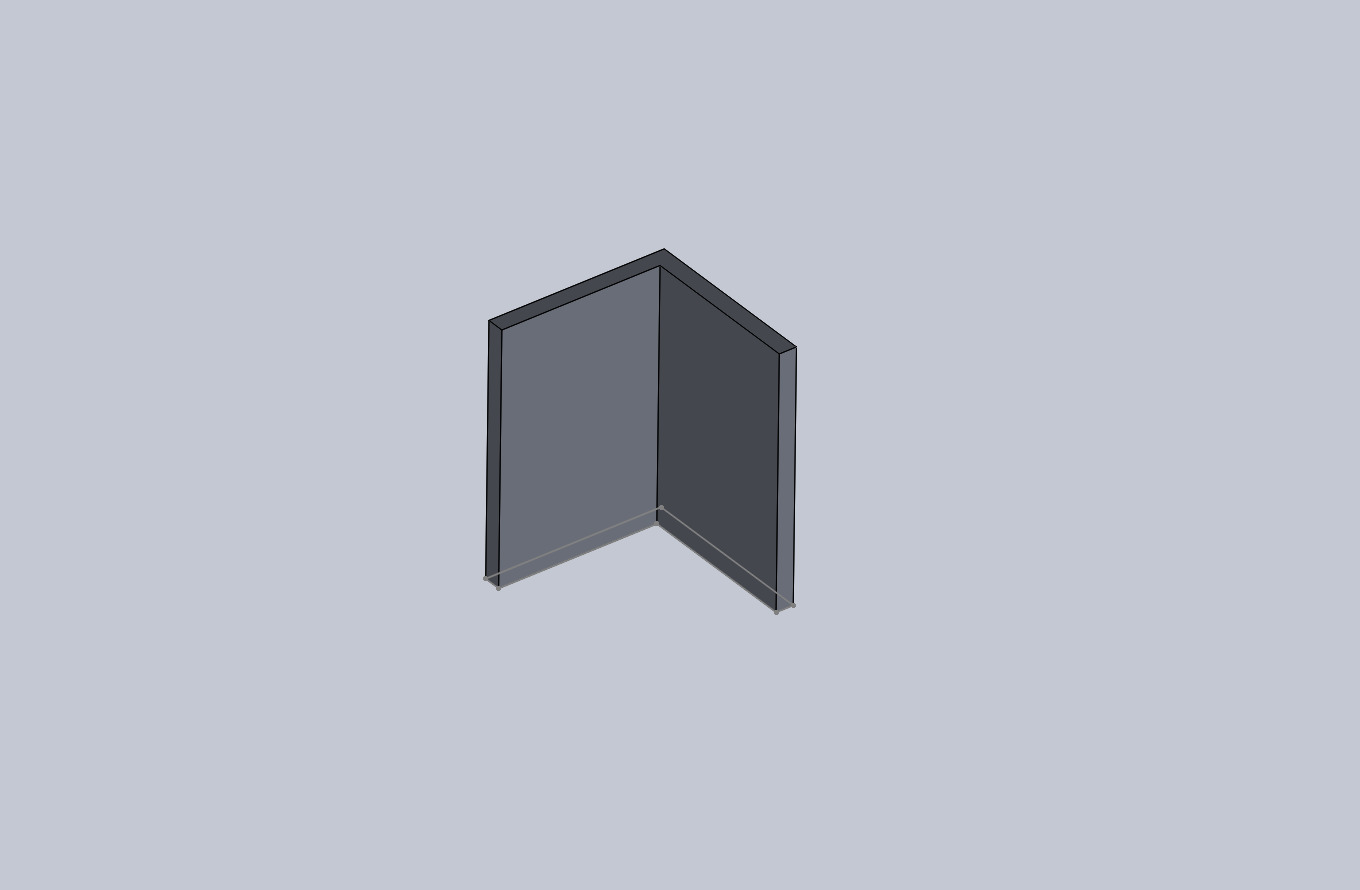
\includegraphics[width=0.5\linewidth]{Angulo aluminio.JPG}
    \caption{Perfil angular de aluminio utilizado como base estructural del módulo.}
    \label{fig:perfil_angular_aluminio}
\end{figure}


\subsubsection{Soporte del motor}
Se conservó el motor NEMA 17 de la configuración original. A partir de sus dimensiones se diseñó un soporte para fijarlo a la base estructural y mantener su alineación con el extrusor MK8. Debido a que el motor y el mecanismo de alimentación se desplazan junto con el carro del eje X, la configuración corresponde a un sistema de extrusión directa. La interfaz diseñada se muestra en la Figura~\ref{fig:soporte_extrusor}.

\begin{figure}[H]
    \centering
    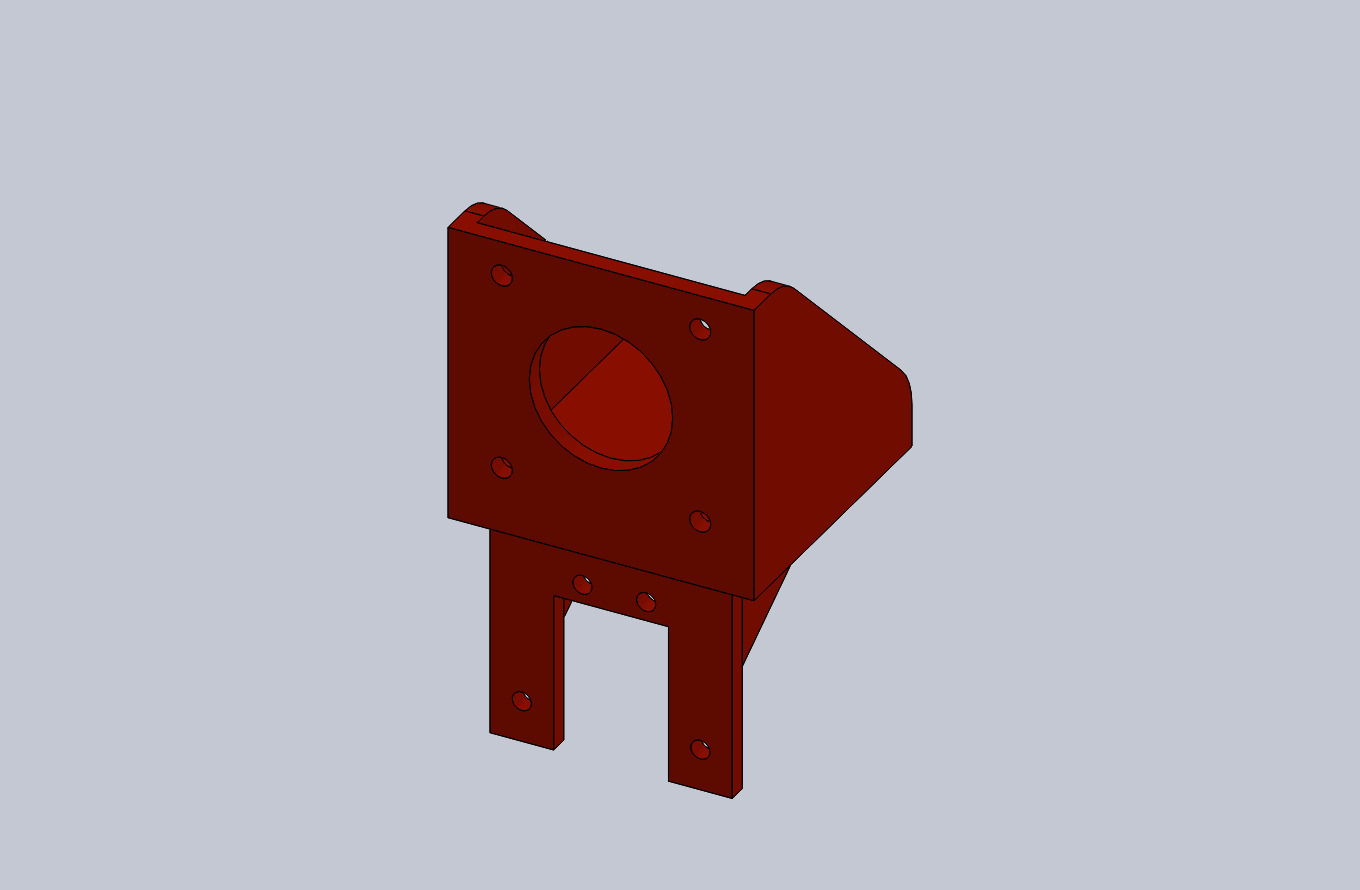
\includegraphics[width=0.5\linewidth]{Soporte ExtrusorV2.JPG}
    \caption{Soporte e interfaz diseñados para el extrusor MK8}
    \label{fig:soporte_extrusor}
\end{figure}
 
\subsubsection{Enfriador de hotend}
\label{subsec:enfriador_hotend}
Para limitar la propagación de calor hacia la zona fría del hotend se diseñó un conducto que dirige aire forzado sobre el disipador. La geometría se definió de manera que el flujo alcanzara las superficies del disipador sin interferir con el desplazamiento de los ejes ni con el sistema independiente de enfriamiento de capa.

\begin{figure}[H]
    \centering
    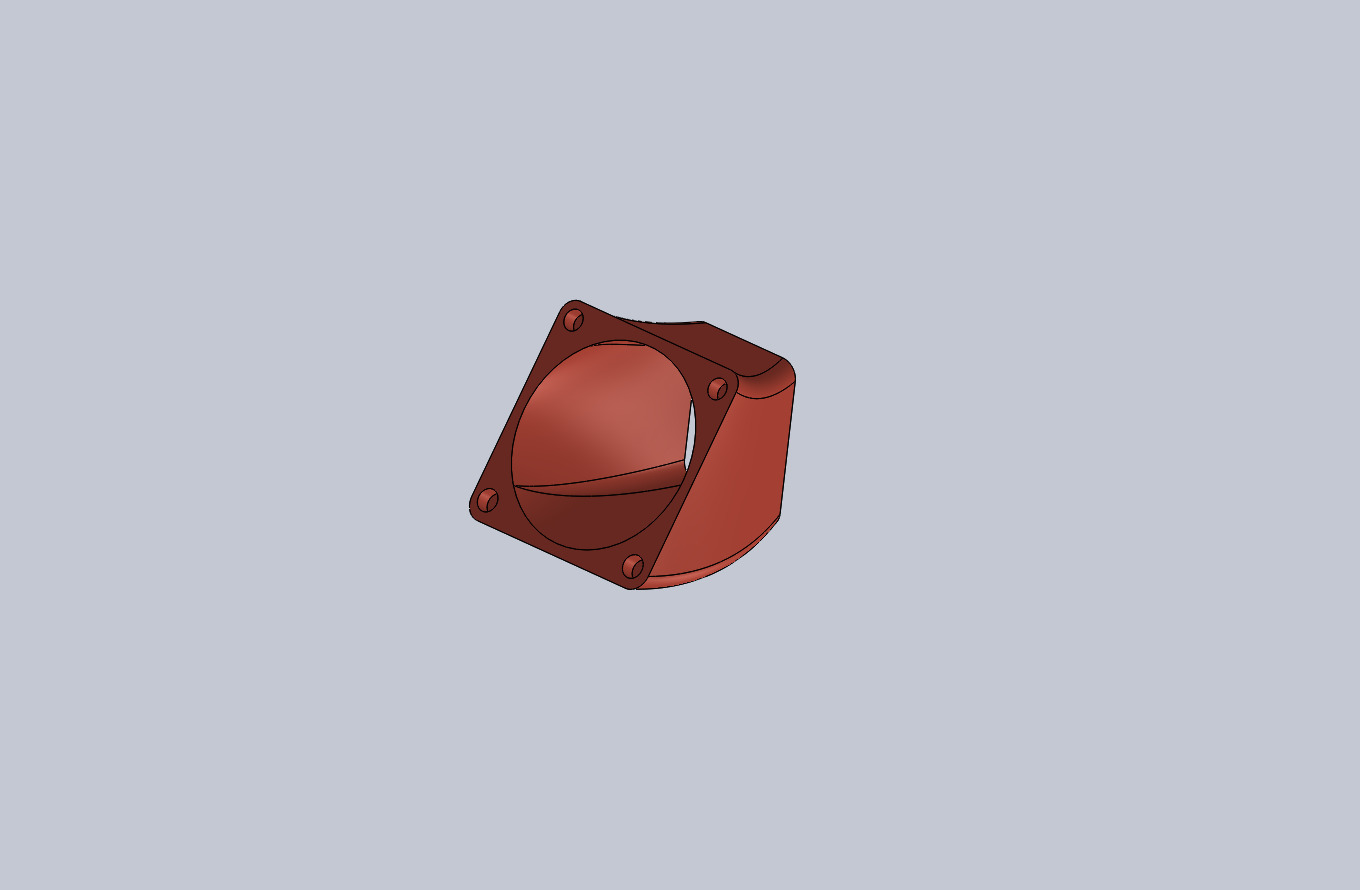
\includegraphics[width=0.5\linewidth]{Enfriador _HotendV2.JPG}
    \caption{Conducto diseñado para el enfriamiento del disipador del hotend.}
    \label{fig:enfriador_hotend}
\end{figure}

\subsubsection{Sistema de enfriamiento de capa}
\label{subsec:enfriamiento_capa}
La configuración original no disponía de ventilación dirigida hacia el material recién depositado Figura~\ref{fig:enfriador_capa}. Por ello se desarrolló un sistema independiente de enfriamiento de capa formado por un ventilador radial de 12 V y un conducto con dos salidas. La geometría dirige el aire hacia la región próxima a la boquilla desde dos lados, procurando evitar la incidencia directa sobre el bloque calefactor.

\begin{figure}[H]
    \centering
    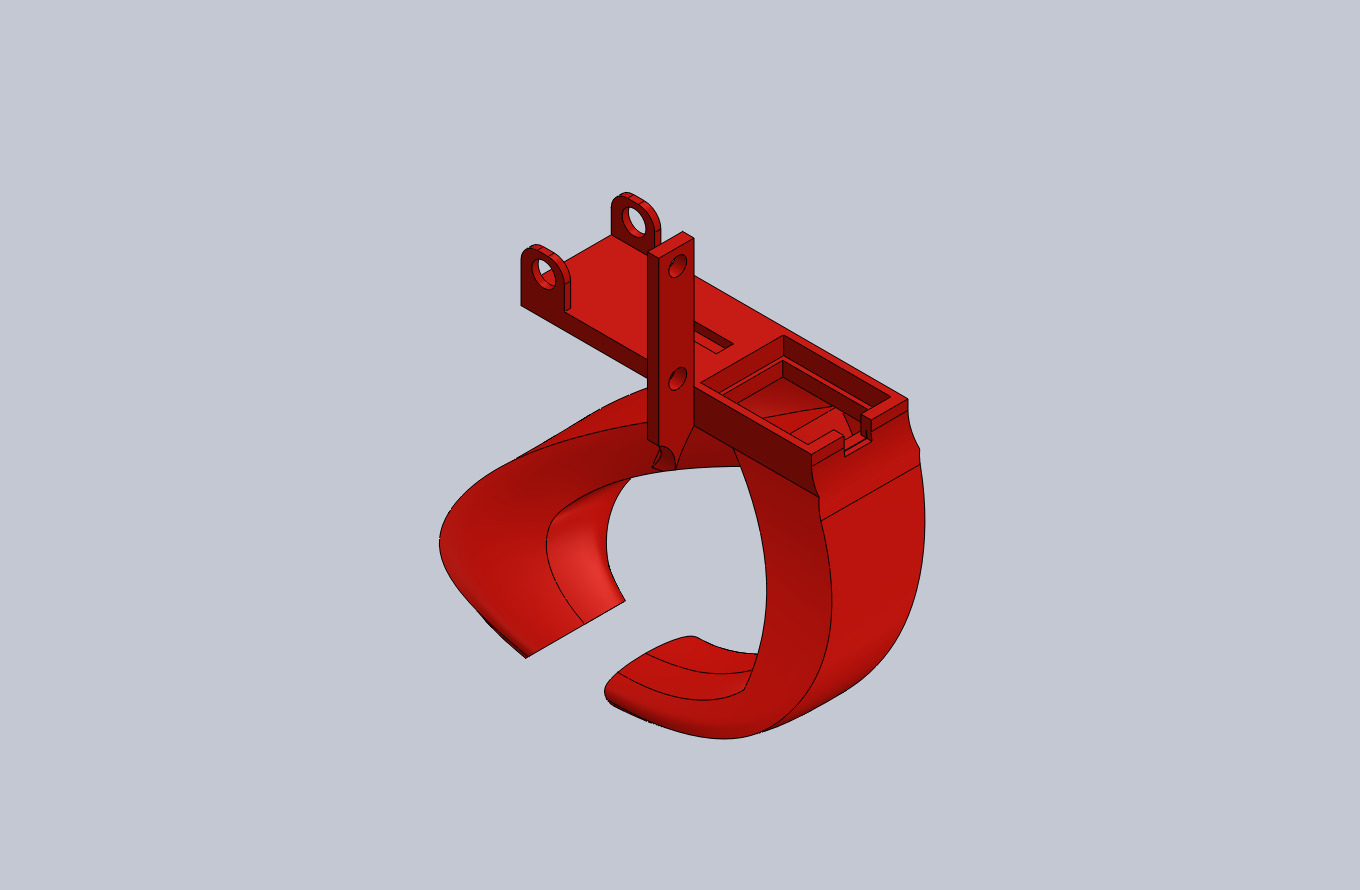
\includegraphics[width=0.5\linewidth]{enfriador de capa2.JPG}
    \caption{Diseño del sistema de enfriamiento de capa}
    \label{fig:enfriador_capa}
\end{figure}

\subsubsection{Modelado y ensamblaje virtual}
Una vez definidos los componentes se realizó un ensamblaje virtual del módulo en SolidWorks. El modelo integró la base de aluminio, el motor, el extrusor MK8, el hotend y ambos sistemas de ventilación. Esta etapa se utilizó para comprobar la posición relativa de los elementos, la alineación del recorrido del filamento y las separaciones necesarias antes de la fabricación e integración física. La
configuración obtenida se muestra en la Figura~\ref{fig:ensamblaje_final_extrusor}.

\begin{figure}[H]
    \centering
    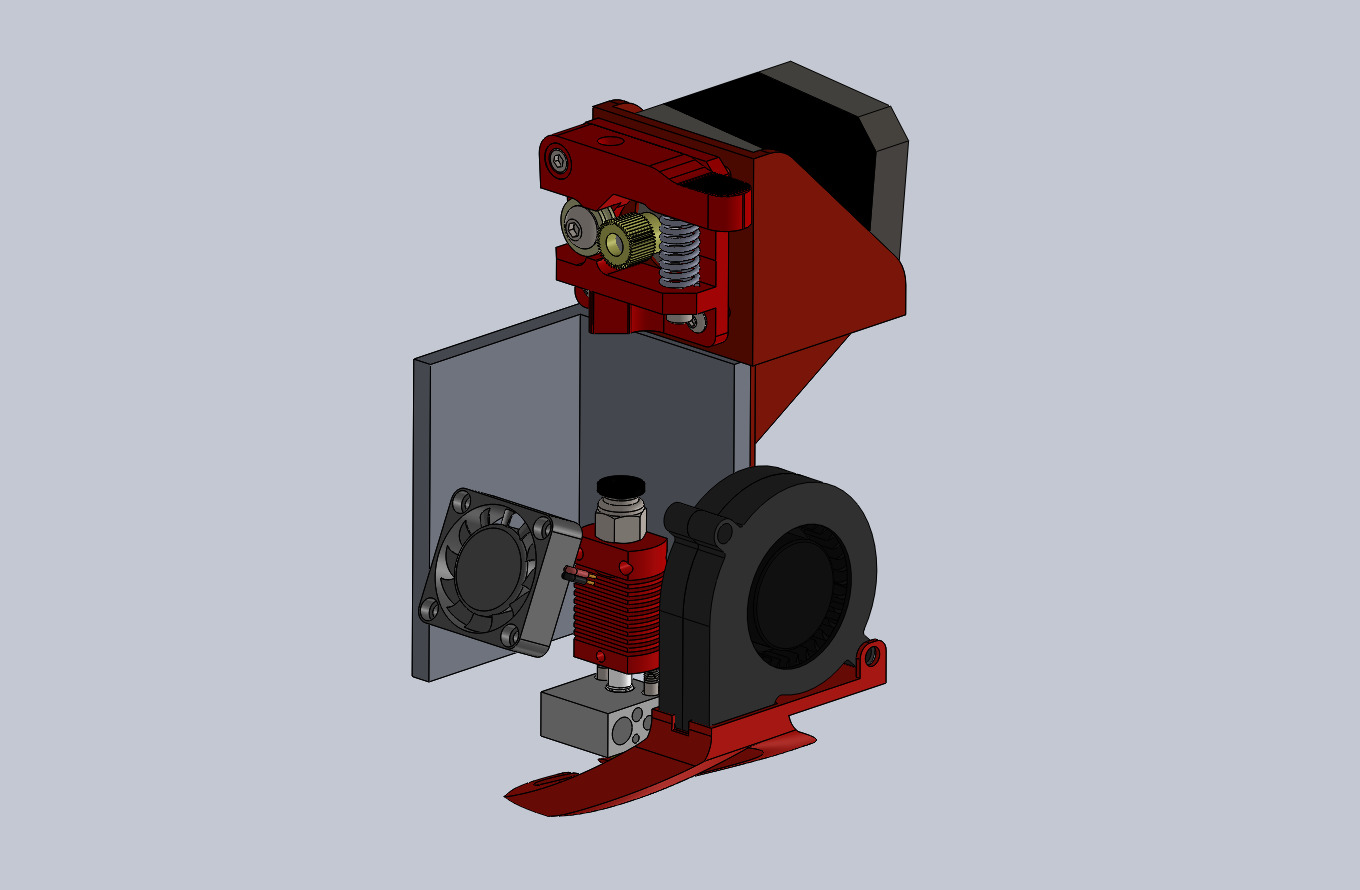
\includegraphics[width=0.5\linewidth]{ensamblaje_final_extrusor.jpg}
    \caption{Ensamble virtual del módulo de extrusión}
    \label{fig:ensamblaje_final_extrusor}
\end{figure}


\subsection{Diseño de componentes auxiliares}
El diagnóstico también mostró limitaciones mecánicas no asociadas directamente con el hotend. Para atenderlas se diseñaron piezas auxiliares orientadas a incrementar la rigidez de determinadas uniones y facilitar los procedimientos de ajuste. Estos componentes se modelaron en SolidWorks y se fabricaron en PLA mediante FDM.

\subsubsection{Escuadras de refuerzo}
En algunas uniones de los perfiles de aluminio se observó juego mecánico. Se diseñaron escuadras de refuerzo para instalarse en los puntos identificados como menos rígidos. La geometría empleada se muestra en la Figura~\ref{fig:estabilizador}.

\begin{figure}[H]
    \centering
    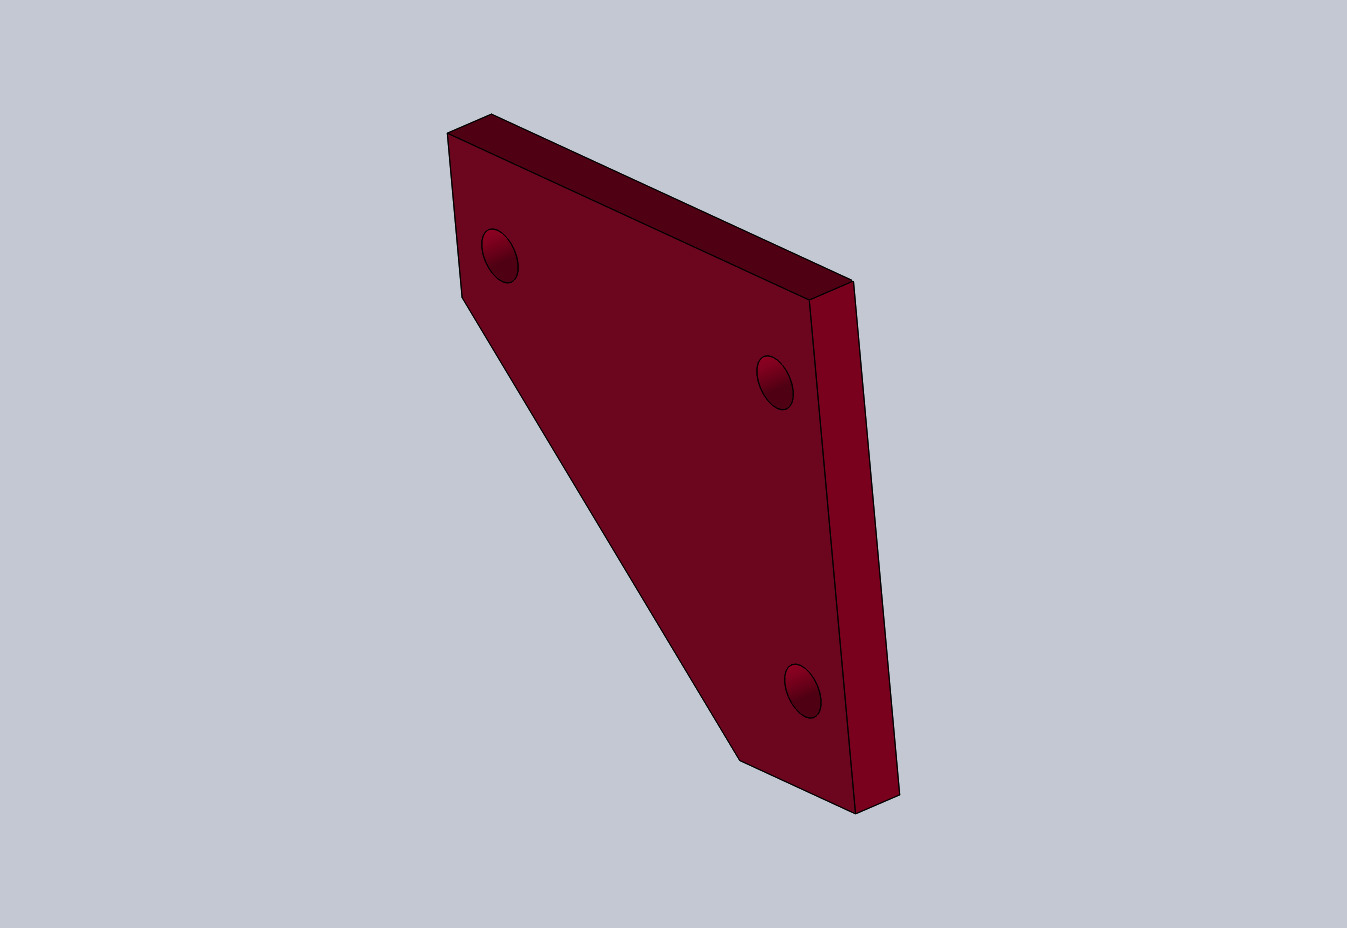
\includegraphics[width=0.5\linewidth]{estabilizador.JPG}
    \caption{Escuadra de refuerzo diseñada para la estructura.}
    \label{fig:estabilizador}
\end{figure}

\subsubsection{Tensor de la correa del eje X}
El ajuste original de la correa del eje X requería modificar manualmente su posición durante el ensamblaje. Para facilitar esta operación se desarrolló un tensor ajustable que permite variar la tensión con el sistema ya montado. La geometría se adaptó a las dimensiones de la plataforma a partir de mecanismos utilizados en proyectos de hardware abierto \cite{placeholder_proyecto_open_source}. El mecanismo diseñado se muestra en la Figura~\ref{fig:tensor_eje_x}.

\begin{figure}[H]
    \centering
    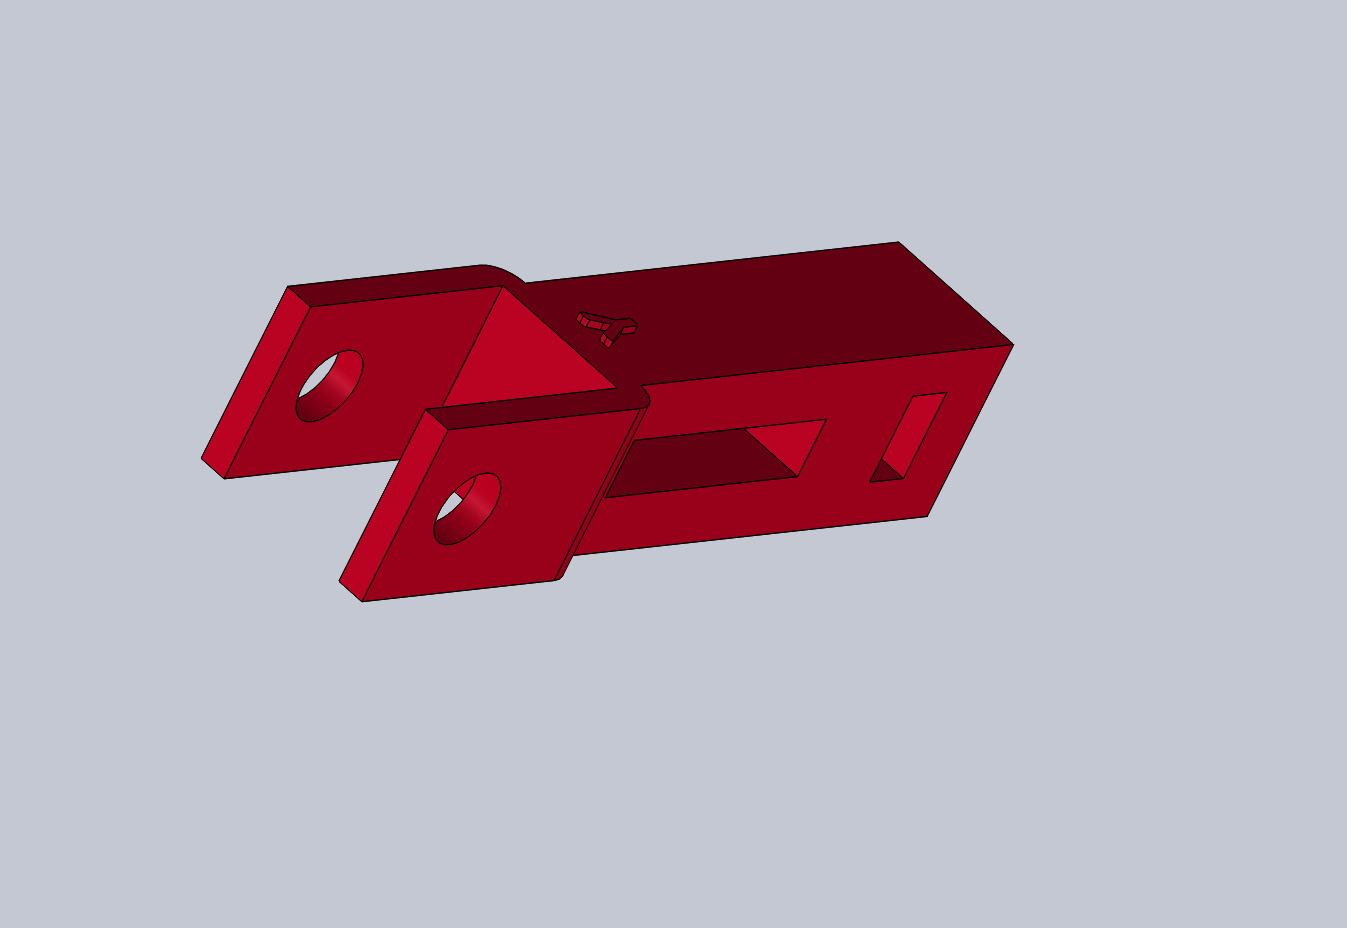
\includegraphics[width=0.5\linewidth]{Estructura de rodamiento Y.JPG}
    \caption{Tensor Eje X}
    \label{fig:tensor_eje_x}
\end{figure}

\subsubsection{Sistema de ajuste para finales de carrera}
También se diseñó un soporte ajustable para los interruptores de límite. El objetivo fue permitir el reposicionamiento del sensor sin desmontar elementos estructurales, de modo que la referencia de origen pudiera corregirse durante la calibración y el mantenimiento. El mecanismo diseñado se muestra en la Figura~\ref{fig:calibrador_altura}.

\begin{comment}
    Como solución se desarrolló un mecanismo de ajuste que permite modificar la posición de los finales de carrera sin necesidad de desmontar componentes estructurales. Este sistema facilita la calibración inicial de la máquina y permite realizar correcciones posteriores de manera rápida y repetible.

La implementación de este elemento contribuyó a mejorar la precisión del proceso de homing y redujo significativamente el tiempo requerido para la puesta en marcha del sistema.
\end{comment}


\begin{figure}[H]
    \centering
    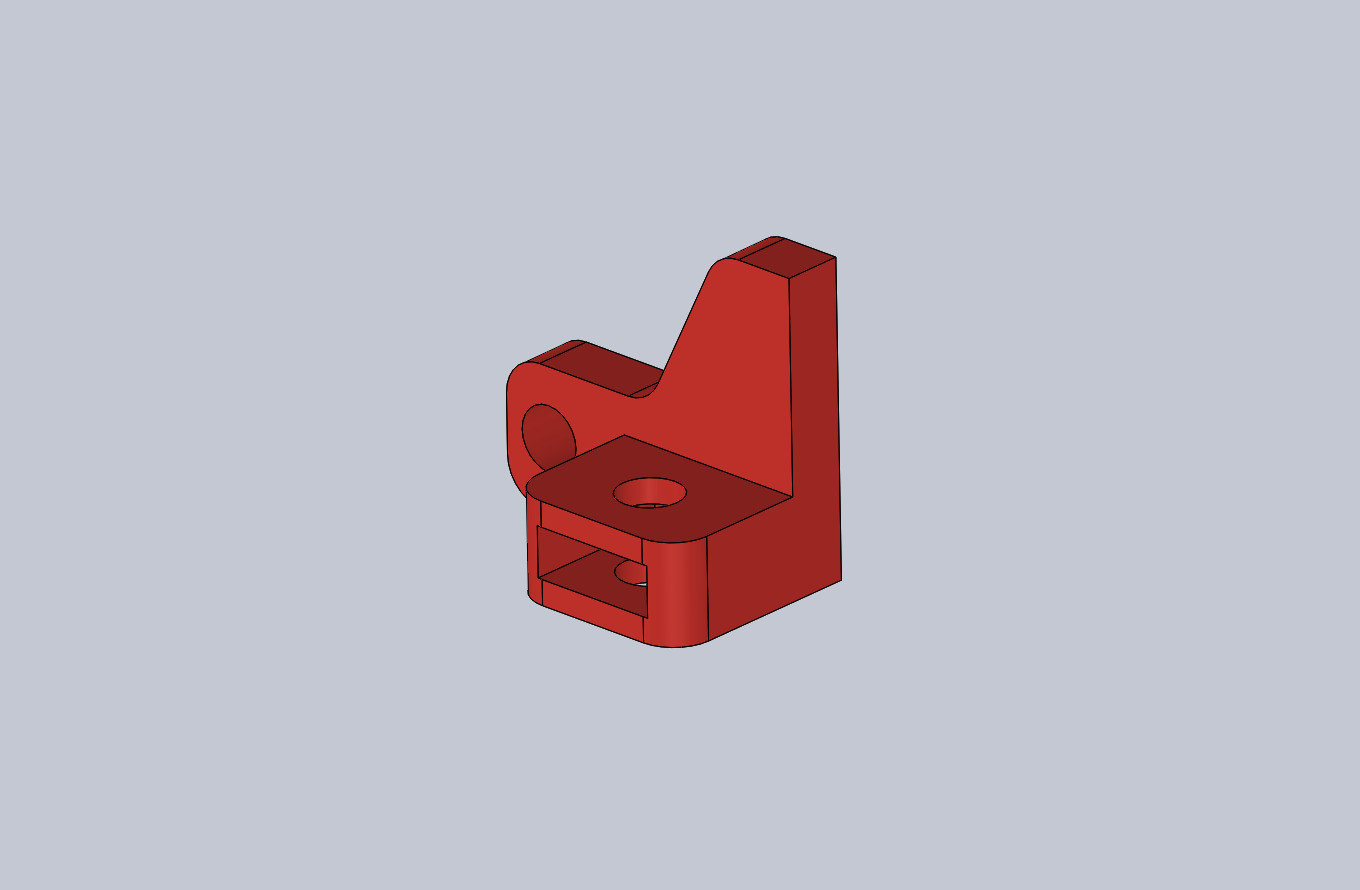
\includegraphics[width=0.5\linewidth]{Calibrador de altura.JPG}
    \caption{Sistema de ajuste para finales de carrera}
    \label{fig:calibrador_altura}
\end{figure}


%%%%%%%%%%%%%%%%%%%%%%%%%%%%%%%%%%%%%%%%%%%%%%%%%%%%%%%%%%%%%%%%%%%%%%%%%%%%%%%%%%%%%%%%%%%%%%%%%%%%%%%%%%%%%%%%%%%%%%%%%%%%%%%%%%%%%%%%%%%%%%%%%%%%%%%%%%%%%%%%%%%%%%%%%%%%%%%%%%%%%%%%%%%%%%%%%%%%%%%%%%%%%%%%%%%%%%%%%%%%%%%%%%%%%%%%%%%%%%%%%%%%%%%%%%%%%%%%%%%%%%%%%%%%%%%%%%%%%%%%%%%%%%%%%%%%%%%%%%%%%%%%%%%%%%%%%%%%%%%%%%%%%%%%%%%%

\section{Materiales y métodos de fabricación}
\subsection{Componentes principales}
Los componentes empleados para la integración de la plataforma se presentan en la Tabla~\ref{tab:materiales_componentes}. La selección del hotend y del sistema de alimentación respondió a su compatibilidad con filamento de \SI{1.75}{\milli\metre}, disponibilidad comercial y facilidad de reemplazo.
\begin{table}[htbp]
    \centering
    \small % Disminuye un poco la fuente para evitar desbordamientos
    \caption{Materiales y componentes utilizados en la fabricación de la impresora.}
    \label{tab:materiales_componentes}
    % \textwidth fuerza a la tabla a no salirse del margen de la página
    \begin{tabularx}{\textwidth}{>{\raggedright\arraybackslash}p{3.8cm} Y l}
        \toprule
        \textbf{Componente} & \textbf{Especificación} & \textbf{Cantidad} \\
        \midrule
        Microcontrolador & Arduino Mega & 1 pza. \\
        Placa de potencia & RAMPS 1.4 & 1 pza. \\
        Motores paso a paso & NEMA 17 (\qty{1.7}{\A}) & 4 pzas. \\
        Cables para motor & Longitud de \qty{1}{\m} & 4 pzas. \\
        Hotend & Ender Creality CR-10, boquilla \qty{0.4}{\mm}, filamento \qty{1.75}{\mm} & 1 pza. \\
        Cama caliente & Dimensión \qty{214}{\mm} $\times$ \qty{214}{\mm}; \qty{12}{\V} / \qty{24}{\V} & 1 pza. \\
        Fuente de poder & \qty{12}{\V} - \qty{30}{\A} (\qty{360}{\W}) & 1 pza. \\
        Controlador de motor & A4988 con disipador térmico & 4 pzas. \\
        Ventilador & \qty{12}{\V}, \qty{40}{\mm} & 2 pzas. \\
        Extrusor & Ender Creality CR-10S & 1 pza. \\
        Resortes para cama & Acero; DE: \qty{9.8}{\mm}, DI: \qty{5.45}{\mm}, Altura: \qty{25.3}{\mm} & 4 pzas. \\
        Tubo de teflón & PTFE translúcido ID: \qty{2}{\mm}, OD: \qty{4}{\mm}, Longitud: \qty{2}{\m} & 1 pza. \\
        Microswitch endstop & Con cable conector, \qty{24}{\V}, \qty{1.6}{\mm} $\times$ \qty{3}{\mm} $\times$ \qty{4}{\mm} & 3 pzas. \\
        Banda dentada & GT2 \qty{6}{\mm} (\qty{1}{\m}) & 2 pzas. \\
        Polea dentada & GT2 20T para banda de \qty{6}{\mm} & 2 pzas. \\
        Termistor & NTC 100K con cable & 2 pzas. \\
        Tubo termorretráctil & Diámetros variados & 1 lote \\
        \bottomrule
    \end{tabularx}
\end{table}





\subsection{Fabricación de piezas poliméricas}

Las piezas de geometría específica se fabricaron mediante FDM utilizando la impresora rehabilitada. Los modelos CAD se exportaron en formato STL y se procesaron en Ultimaker Cura 5.12. Se utilizó filamento PLA de 1.75 mm y boquilla de 0.4 mm.

La orientación de cada pieza se seleccionó considerando las superficies de apoyo, la geometría y la dirección principal de las cargas durante su funcionamiento. Cuando la geometría lo requirió se utilizaron estructuras de soporte. Después de la impresión se inspeccionaron las piezas para detectar deformaciones, separación entre capas o formación excesiva de hilos; posteriormente se retiraron soportes y se limpiaron las superficies y orificios destinados al montaje.

Los valores definitivos de altura de capa, temperatura de extrusión, temperatura de cama y patrón de relleno deben registrarse a partir de los archivos de laminado empleados durante la fabricación. No se incorporan valores no documentados en los registros del proyecto. La densidad de relleno registrada para las piezas finales fue de 40 $\%$ y la velocidad de impresión de 50 mm/s.

\subsection{Fabricación de la base metalica}

La base estructural del módulo se fabricó a partir de un perfil angular de aluminio de 4 mm de espesor. Se cortó una sección de 100 mm y posteriormente se trazaron y perforaron los puntos de montaje correspondientes a tornillos M3. Después del corte y perforado se eliminaron rebabas y se ajustaron los bordes mediante esmerilado. Antes del montaje final se verificó la correspondencia de los orificios con el motor, el hotend y los soportes.

\subsection{Integración del módulo de extrusión }

La base de aluminio se instaló sobre el carro del eje X. Sobre ella se montaron el motor NEMA 17, el mecanismo MK8 y el hotend, verificando la alineación del recorrido del filamento. Posteriormente se instalaron el ventilador axial destinado al disipador del hotend y el ventilador radial utilizado para el enfriamiento de capa, junto con sus respectivos conductos.

También se incorporaron el cartucho calefactor, el termistor y los conductores eléctricos necesarios para la conexión con la tarjeta de control. Antes de energizar los calentadores se verificó manualmente el avance del filamento, la sujeción de los componentes y la ausencia de interferencias entre el módulo y la estructura durante el desplazamiento del carro.

\section{Configuración y calibración}

Concluido el ensamblaje se configuró el sistema de control y se calibraron los mecanismos de movimiento, la alimentación de filamento y el control térmico. Estas actividades se realizaron antes de las pruebas de impresión con el propósito de establecer parámetros de operación reproducibles.

\subsection{Configuración del firmware REVISAR}
La electrónica utiliza un Arduino Mega con tarjeta RAMPS 1.4. Sobre esta plataforma se instaló Marlin 2.1.2.1 \cite{marlinfw} y se configuraron desde cero los parámetros correspondientes a los ejes X, Y y Z, el extrusor, los sensores de temperatura, los calentadores, los ventiladores y los interruptores de límite.

Los valores iniciales de pasos por unidad se calcularon a partir de las características de los motores y de los mecanismos de transmisión. Antes de activar los calentadores se comprobaron individualmente los movimientos de los ejes, verificando el sentido de desplazamiento, la actuación de los finales de carrera y la ausencia de interferencias mecánicas.

\subsection{Calibración del sistema de movimiento}
\label{sec:calibracion_del_sistema_de_movimiento}

Para verificar la correspondencia entre desplazamiento programado y desplazamiento real se realizaron pruebas independientes en X, Y y Z. En cada eje se ordenaron diez desplazamientos consecutivos de 10 mm en el mismo sentido, equivalentes a 100 mm programados. La distancia total recorrida se midió y se comparó con la solicitada.
Cuando se detectó una diferencia, el parámetro de pasos por milímetro se corrigió mediante la relación:

\begin{equation}
E_{\mathrm{nuevo}} = E_{\mathrm{actual}} \cdot 
\frac{L_{\mathrm{programada}}}{L_{\mathrm{medida}}}
\label{eq:pasos_mm_movimiento}
\end{equation}



donde $E_{\mathrm{nuevo}}$ corresponde al nuevo valor de pasos por milímetro 
del eje, $E_{\mathrm{actual}}$ al valor utilizado durante la prueba, 
$L_{\mathrm{programada}}$ a la distancia solicitada y $L_{\mathrm{medida}}$ a 
la distancia realmente recorrida. Los valores finales y el
error medido se presentan en el capítulo de resultados.

\subsection{Calibración del extrusor}
\label{sec:calibracion_extrusor}
La calibración del extrusor se realizó para establecer la correspondencia entre la longitud de filamento solicitada y la longitud realmente suministrada. Para aislar la respuesta del mecanismo de alimentación se retiró el hotend durante esta prueba. Se marcó una referencia sobre el filamento y se ordenaron diez desplazamientos de 10 mm, equivalentes a una alimentación total programada de 100 mm.

La longitud desplazada se midió desde la referencia inicial y el valor de pasos por milímetro se corrigió mediante la ecuación~\ref{eq:pasos_mm_movimiento}, sustituyendo el desplazamiento del eje por la longitud de filamento. Después de incorporar el nuevo valor al firmware se realizó una prueba adicional de verificación.

\subsection{Ajuste del control térmico}
\label{sec:calibracion_termica}
La regulación térmica se ajustó para el hotend y la cama calefactada utilizando la función de autosintonización PID disponible en Marlin. El procedimiento se ejecutó de manera independiente para cada elemento a las temperaturas de operación utilizadas para PLA. Las constantes obtenidas se incorporaron a la configuración del firmware.

Después de la sintonización se verificó el comportamiento térmico durante la operación de la impresora. Las constantes finales, las temperaturas alcanzadas, los tiempos de calentamiento y la variación en estado estable se presentan en el capítulo de resultados.

\section{Protocolo de evacuación experimental}
Una vez configurada y calibrada la plataforma se estableció un conjunto de pruebas para evaluar el sistema final. Los resultados se reservan para el capítulo siguiente; en esta sección se definen únicamente las variables y procedimientos de medición.

\subsection{Evaluación del posicionamiento y la extrusión}
La precisión de movimiento se evaluó comparando distancias programadas con distancias medidas en cada eje. Para el extrusor se comparó una longitud programada de filamento con la longitud efectivamente suministrada. En ambos casos se calculó el error absoluto y el error relativo porcentual respecto al valor programado. 

\subsection{Evacuación térmica}
Para el hotend y la cama se registraron la temperatura programada, la temperatura alcanzada, el tiempo necesario para alcanzar la condición de operación y la variación observada una vez alcanzado el régimen estable. Para evaluar el sistema de disipación del hotend se realizaron mediciones de temperatura en el disipador manteniendo constante la temperatura del bloque calefactor y modificando la configuración de ventilación. La posición del sensor se mantuvo fija entre pruebas para conservar condiciones comparables.

\subsection{Evaluación dimensional y de calidad de impresión}
La precisión dimensional se evaluó mediante piezas de geometría conocida. Las dimensiones obtenidas se midieron sobre los ejes X, Y y Z y se compararon con las dimensiones nominales del modelo. El análisis se complementó con una inspección visual de defectos de impresión, incluyendo presencia de hilos, deformación de la base y patrones asociados con vibración.

También se contemplaron pruebas geométricas destinadas a observar el comportamiento en voladizos, puentes y movimientos con retracción. Las condiciones de laminado utilizadas en cada ensayo deben mantenerse registradas para permitir una comparación reproducible entre las piezas.

\subsection{Evacuación económica}
La evaluación económica se planteó a partir del costo de los componentes utilizados en la construcción e integración de la plataforma. Para la comparación con alternativas comerciales se considerarán equipos con volumen de impresión y aplicación general comparables. El costo de mano de obra no se incorpora al costo de fabricación, ya que el diseño, ensamblaje y calibración fueron realizados por el autor como parte del trabajo académico. Los precios, modelos comerciales y fecha de consulta se presentan en el capítulo de resultados.

\section{Resumen del capitulo}
El procedimiento descrito permitió pasar de una plataforma fuera de servicio a una configuración rehabilitada, diagnosticada y posteriormente modificada mediante un proceso iterativo de diseño. Las intervenciones se concentraron en el módulo de extrusión, el manejo térmico, el enfriamiento de capa y los mecanismos auxiliares de ajuste. Después de la integración se configuraron y calibraron los subsistemas mecánicos, de extrusión y térmicos, y se definió un protocolo para evaluar el desempeño del sistema. El capítulo siguiente presenta los resultados obtenidos mediante estos procedimientos
